\section{INTRODUCCION} 

\begin{enumerate}[1.]
	\item Introduccion:

A lo largo de estos años hemos visto surgir el Desarrollo de Software Dirigido por Modelos (MDD) como una nueva área dentro el campo de
la ingeniería de software. MDD plantea una nueva forma de entender el desarrollo y mantenimiento de sistemas de software con el uso de modelos como principales artefactos del proceso de desarrollo. En MDD, los modelos son utilizados para dirigir las tareas de comprensión, diseño, construcción, pruebas, despliegue, operación, administración, mantenimiento y modificación de los sistemas. En este libro explicamos los fundamentos de MDD, respondiendo a preguntas tales como “¿Qué son los modelos, cómo se construyen y cómo se transforman hasta llegar al código ejecutable?”. También nos referimos a los estándares que soportan a MDD y discutimos las ventajas
que se introducen en el ciclo de vida del software como consecuencia de adoptarlo. El libro contiene un ejemplo completo de un desarrollo dirigido por modelos. El desarrollo comienza con la definición de un modelo abstracto expresado en UML y finaliza con el despliegue de un programa ejecutable escrito en Java. La transformación del modelo a código es realizada a través de la aplicación de transformaciones expresadas en un lenguaje estándar. Este ejemplo brinda un panorama completo y comprensible sobre los aspectos técnicos de MDD.
¿A quién está dirigido este lib

\begin{center}
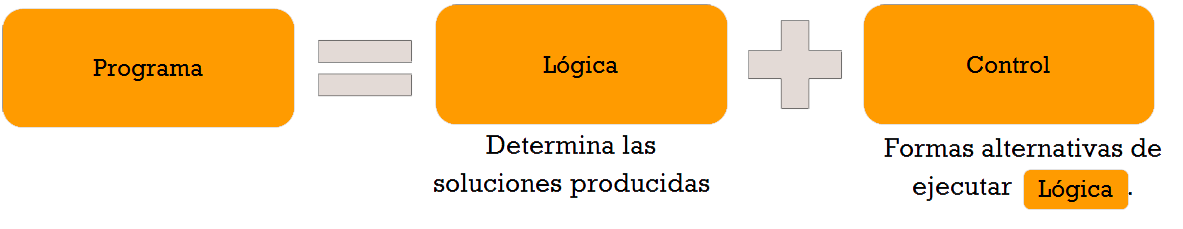
\includegraphics[scale=0.40]{./Imagenes/img02.png} 
\end{center}